\documentclass[a4paper]{article}

\usepackage{polski}
\usepackage[utf8]{inputenc}

\usepackage[export]{adjustbox}
\usepackage{scrextend}
\usepackage{amsfonts}
\usepackage{amsmath}
\usepackage{svg}

\usepackage{geometry}
\geometry{a4paper, left=15mm, top=30mm, right=15mm, bottom=20mm}

\usepackage{gensymb}
\usepackage{graphicx} 
\usepackage{isotope}
\usepackage{array}
\usepackage{float}
\usepackage{titlesec}
\usepackage{fancyhdr}
\usepackage{multirow}

\usepackage{hyperref}
\usepackage{sectsty}
\usepackage{enumitem}
\usepackage{listings}
\usepackage[labelformat=simple]{subcaption}
\usepackage{xcolor,colortbl}
\usepackage{animate}

\sectionfont{\normalfont\huge\sectionrule{0pt}{0pt}{-6pt}{1pt}}
\subsectionfont{\normalfont\LARGE}

\pagestyle{fancy}
\fancyhf{}
\fancyhead[LE,LO]{\Large Łukasz Kwinta, Kacper Kozubowski, Ida Ciepiela}
\fancyhead[LE,RO]{\Large Transkoder liczb}
\fancyfoot[CE,CO]{\Large\thepage}

\renewcommand{\footrulewidth}{1pt}
\renewcommand{\headrulewidth}{1pt}

\definecolor{Gray}{gray}{0.85}
\definecolor{LightGray}{gray}{0.95}

\newcolumntype{a}{>{\columncolor{Gray}}c}
\newcolumntype{b}{>{\columncolor{white}}c}

\hypersetup{
    colorlinks,
    citecolor=black,
    filecolor=black,
    linkcolor=black,
    urlcolor=black
}

\title{\fontsize{30pt}{30pt}\selectfont Laboratorium 1 \\ Transkoder liczb}
\author{\fontsize{20pt}{20pt}\selectfont Łukasz Kwinta, Kacper Kozubowski, Ida Ciepiela}
\date{marzec 2024}

\begin{document}
\maketitle
\newpage
\section{Cel zadania}
\Large Celem zadania było zaprojektować,
 zbudować i przetestować układ kombinacyjny realizujący transkoder czterobitowej liczby naturalnej (wraz z zerem)
  na sześciobitową liczbę pierwszą, bazując wyłącznie na bramkach NAND.

\section{Idea rozwiązania}
\Large Nasze rozwiązanie opiera się na przekształcaniu 4 bitów wejściowych za pomocą transkoderów, generując w rezultacie 6 bitów wyjściowych.
 Aby uzyskać konkretne kombinacje bitów wyjściowych, zastosowaliśmy funkcje logiczne opracowane z wykorzystaniem tablic Karnaugh.

\section{Układ transkodera liczb pierwszych}
\subsection{Black box}
Pierwszym krokiem w projektowaniu układu jest przedstawienie go jako tzw. "Black Box". Czyli taką czarną skrzynkę dla której 
określamy tylko wejście i oczekiwany wynik działania dla danego wejścia ale nie wgłębiamy się w implementację.

\begin{figure}[H]
  \centering
  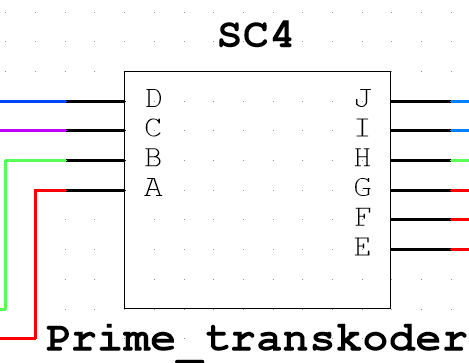
\includegraphics{black_box.png}
\end{figure}

Wejście do układu stanowią 4 piny ABCD kodujące binarnie wejściową liczbę 0-15. Stan wysoki na pinach
stanowi logiczną jedynkę (1), a stan niski logiczne zero (0).
\begin{center}
  \begin{tabular}{|c|c|c|c|c|}
    \hline Numer bitu & 3 & 2 & 1 & 0 \\ 
    \hline Bit & A & B & C & D \\
    \hline Mnożnik & $2^3$ & $2^2$ & $2^1$ & $2^0$  \\
    \hline
  \end{tabular}
\end{center}

Wyjście układu stanowi 6 pinów EFGHIJ kodujące pierwsze 16 liczb pierwszych. Tak samo jak na wejściu stan wysoki na pinach
stanowi logiczną jedynkę (1), a stan niski logiczne zero (0). 
\begin{center}
  \begin{tabular}{|c|c|c|c|c|c|c|}
    \hline Numer bitu & 5 & 4 & 3 & 2 & 1 & 0 \\ 
    \hline Bit & E & F & G & H & I & J \\
    \hline Mnożnik & $2^5$ & $2^4$ & $2^3$ & $2^2$ & $2^1$ & $2^0$ \\
    \hline
  \end{tabular}
\end{center}

Układ mapuje wejście na wyjście w następujący sposób - zakładając notację binarną zapisanego mapowania.

\begin{center}
  \begin{tabular}{|c|c|c|c|c|c|c|c|c|c|c|c|c|c|c|c|c|c|}
    \hline Wejście            & 0 & 1 & 2 & 3 & 4  & 5 & 6 & 7 & 8 & 9 & 10 & 11 & 12 & 13 & 14 & 15 \\ 
    \hline Oczekiwane wyjście & 2 & 3 & 5 & 7 & 11 & 13 & 17 & 19 & 23 & 29 & 31 & 37 & 41 & 43 & 47 & 43 \\ 
    \hline
  \end{tabular}
\end{center}

\subsection{Tabela prawdy}
Poniżej zapisaliśmy tabelę prawd dla projektowanego układu:

\begin{center}
  \begin{tabular}{|c|c|c|c||c|c|c|c|c|c|}
  \hline \multicolumn{4}{|c||}{Wejście} & \multicolumn{6}{|c|}{Wyjście} \\
  \hline A & B & C & D & E & F & G & H & I & J \\
  \hline 0 & 0 & 0 & 0 & 0 & 0 & 0 & 0 & 1 & 0 \\
  \hline 0 & 0 & 0 & 1 & 0 & 0 & 0 & 0 & 1 & 1 \\
  \hline 0 & 0 & 1 & 0 & 0 & 0 & 0 & 1 & 0 & 1 \\
  \hline 0 & 0 & 1 & 1 & 0 & 0 & 0 & 1 & 1 & 1 \\
  \hline 0 & 1 & 0 & 0 & 0 & 0 & 1 & 0 & 1 & 1 \\
  \hline 0 & 1 & 0 & 1 & 0 & 0 & 1 & 1 & 0 & 1 \\
  \hline 0 & 1 & 1 & 0 & 0 & 1 & 0 & 0 & 0 & 1 \\
  \hline 0 & 1 & 1 & 1 & 0 & 1 & 0 & 0 & 1 & 1 \\
  \hline 1 & 0 & 0 & 0 & 0 & 1 & 0 & 1 & 1 & 1 \\
  \hline 1 & 0 & 0 & 1 & 0 & 1 & 1 & 1 & 0 & 1 \\
  \hline 1 & 0 & 1 & 0 & 0 & 1 & 1 & 1 & 1 & 1 \\
  \hline 1 & 0 & 1 & 1 & 1 & 0 & 0 & 1 & 0 & 1 \\
  \hline 1 & 1 & 0 & 0 & 1 & 0 & 1 & 0 & 0 & 1 \\
  \hline 1 & 1 & 0 & 1 & 1 & 0 & 1 & 0 & 1 & 1 \\
  \hline 1 & 1 & 1 & 0 & 1 & 0 & 1 & 1 & 1 & 1 \\
  \hline 1 & 1 & 1 & 1 & 1 & 1 & 0 & 1 & 0 & 1 \\

  \hline 
  \end{tabular}
\end{center}


\subsection{Tablice Karnaugh}
\subsection{Implementacja}

\section{Zastosowania}
Poniżej wymieniamy przykładowe zastosowania zaprojektowanego układu:
\begin{itemize}
  \item Transkoder generujący liczby pierwsze na podstawie prostej liczby może być zastosowany w urządzeniach 
      szyfrujących. Dużo łatwiej jest wygenerować (pseudo)-losową liczbę z przedziału 0-15 i ją przekształcić na
      liczbę pierwszą za pomocą takiego transkodera niż wybierać losową liczbę pierwszą. Wiele algorytmów szyfrujących
      czy funkcji hashujących bazuje na liczbach pierwszych więc taki układ miałby tam zastosowanie.
  \item Innym zastosowaniem układów z rodziny transkoderów - lecz nie koniecznie tego konkretnego - może być 
      przekształcenie kodu jakiegoś błędu reprezentowanego w systemie przez liczby 0-15 na jakiś inny kod błędu, 
      który np. nadaje się do wyświetlenia użytkownikowi - bo mówi coś więcej o istocie problemu.
\end{itemize}
\end{document}